%--------------------------------------------
% Chapter: UDP-BASED NETWORK CONNECTION TO MATLAB
%--------------------------------------------
\chapter{UDP-based network connection to MATLAB}
\label{sec:udpMatlab}

%- - - - - - - - - - - - - - - - - - - - - - 
% Section: C-Library to send and receive sensor and filter data
%- - - - - - - - - - - - - - - - - - - - - - 
\section{C-Library for UDP-based network access}
\label{sec:udpMatlab:udpLib}

To assist and ease the development of the sensor fusion of the IMU data (see chapter \ref{sec:sensorFusion}), a dedicated C-Library for a UDP-based network connection to MATLAB has been implemented. This way, raw and fusioned data can be displayed and processed in a convenient way by using MATLAB/Simulink.

The library \texttt{udpLib} is also capable to enrich all data packets with a precise timestamp according to the \texttt{POSIX.1b} specification. This specification defines a structure composed of a two \texttt{long int} values, as shown in listing \ref{code:udpMatlab:udpLib:posix1b}. The first value stores the elapsed seconds since \texttt{Epoch} (Unix timestamp, seconds elapsed since January 1st, 1970). The second value stores the nanoseconds elapsed since the start of the current second.

\begin{lstlisting}[caption=C-Code snippet of a POSIX.1b conform time specification structure,label=code:udpMatlab:udpLib:posix1b]
struct timespec
{
	long int tv_sec;		/* Seconds since Epoch.  */
	long int tv_nsec;		/* Nanoseconds.  */
};
\end{lstlisting}
\textbf{Important remark:} At the current state, there is \textbf{no} automatic time synchronization between local and remote machine implemented in the library \texttt{udpLib}!

To acquire the precise timestamps, the external library \texttt{librt} has to be linked to the Eclipse Project that utilizes \texttt{udpLib}. Otherwise, a linking error will occur during compilation time.

\subsection{Adding librt to the cross-compiler's linker}
\label{sec:udpMatlab:udpLib:linkerSetup}

To add \texttt{librt} in Eclipse, navigate in the menu to \texttt{Project -> Properties}. A new window will appear as depicted in fig. \ref{fig:udpMatlab:udpLib:eclipseSettings}. At the very left, select \texttt{C/C++ Build} and expand the menu to click on \texttt{Settings}. In the window on the right, there will show up a tabular menu. Select the tab \texttt{Tool Settings} and navigate to \texttt{Cross G++ Linker -> Libraries}.

\begin{figure}[H]
    \centering
    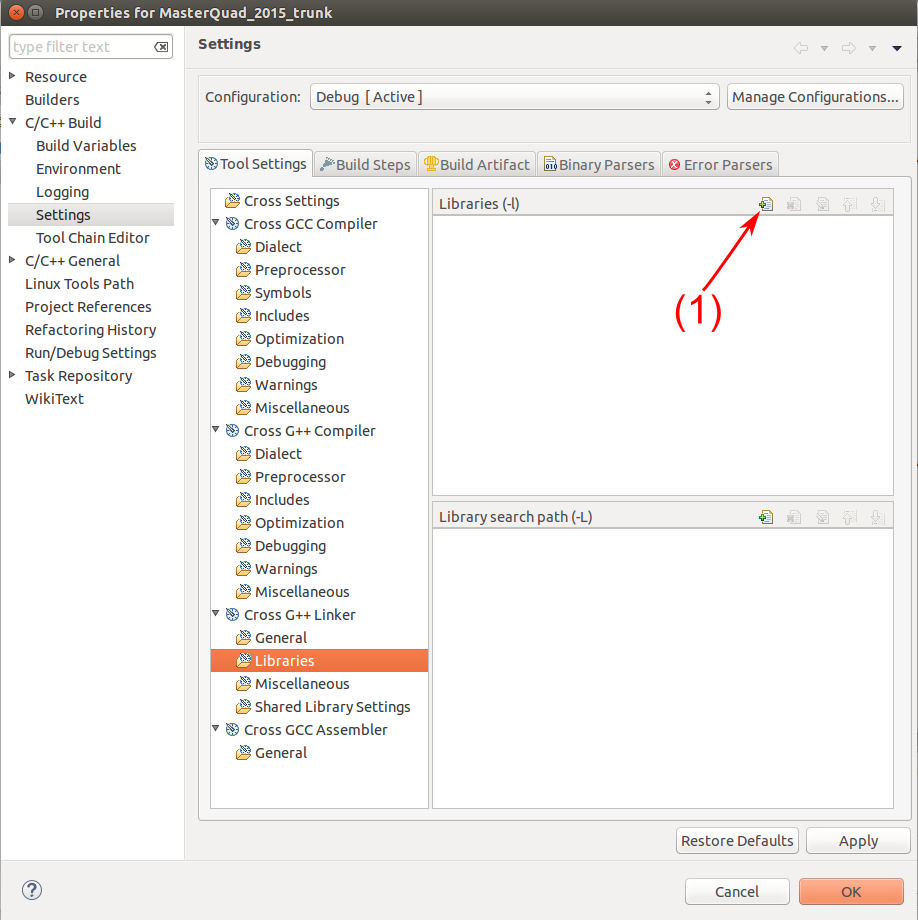
\includegraphics[width=0.5\textwidth]{fig/ch-matlab-lib/projectSettings}
    \caption[Settings menu of Eclipse]{Settings menu window of Eclipse to add the library \texttt{librt} to the cross-compilers linker}
    \label{fig:udpMatlab:udpLib:eclipseSettings}
\end{figure}

In the right, a two-folded textbox with the heading \texttt{Libraries (-l)} and \texttt{Library search path (-L)} will appear. Click on the Plus-Icon of the upper textbox (\texttt{Libraries (-l)}) as indicates with the red arrow in fig. \ref{fig:udpMatlab:udpLib:eclipseSettings}.

\begin{figure}[H]
    \centering
    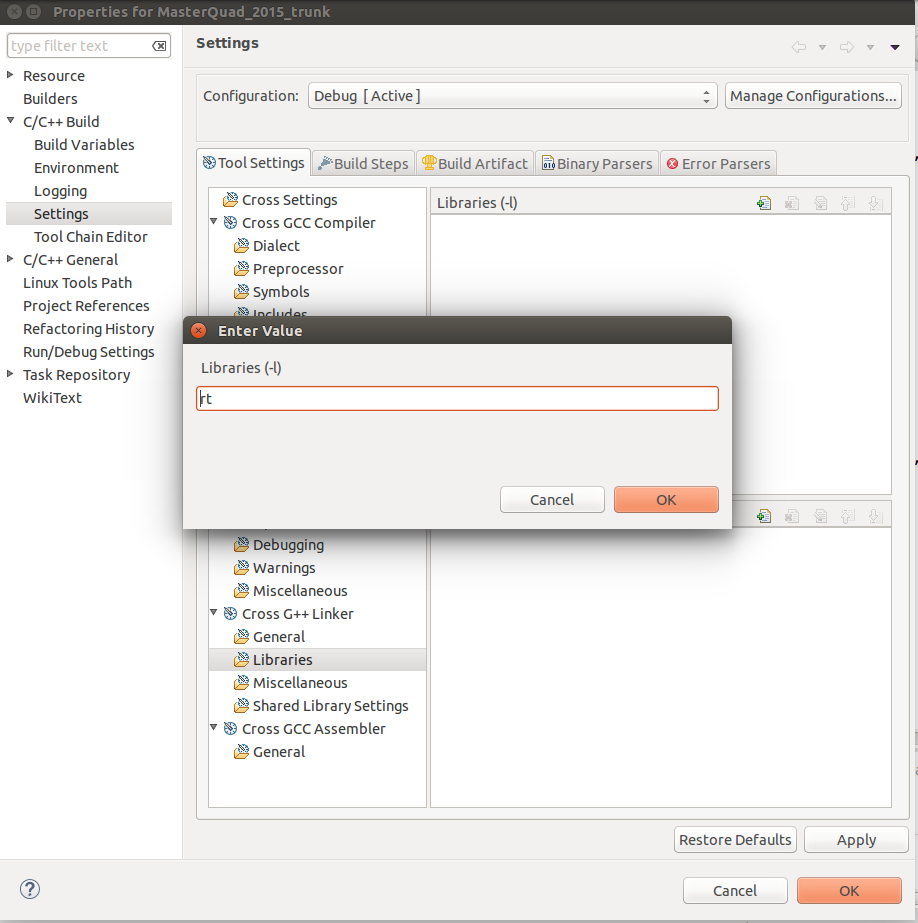
\includegraphics[width=0.5\textwidth]{fig/ch-matlab-lib/projectAddRt}
    \caption[Adding librt to the linker]{Adding the library \texttt{librt} to the cross-compilers linker}
    \label{fig:udpMatlab:udpLib:addLibSettings}
\end{figure}

In consequence, a input window will appear as shown in fig. \ref{fig:udpMatlab:udpLib:addLibSettings}. Type '\texttt{rt}' into the input field and press 'Ok'. Now the textbox \texttt{Libraries (-l)} has a new entry called \texttt{rt} (compare with fig. \ref{fig:udpMatlab:udpLib:addDoneSettings}). Eclipse is now ready to compile and link \texttt{udpLib} successfully. Finally, close the settings window by pressing the Ok-Button.

\begin{figure}[H]
    \centering
    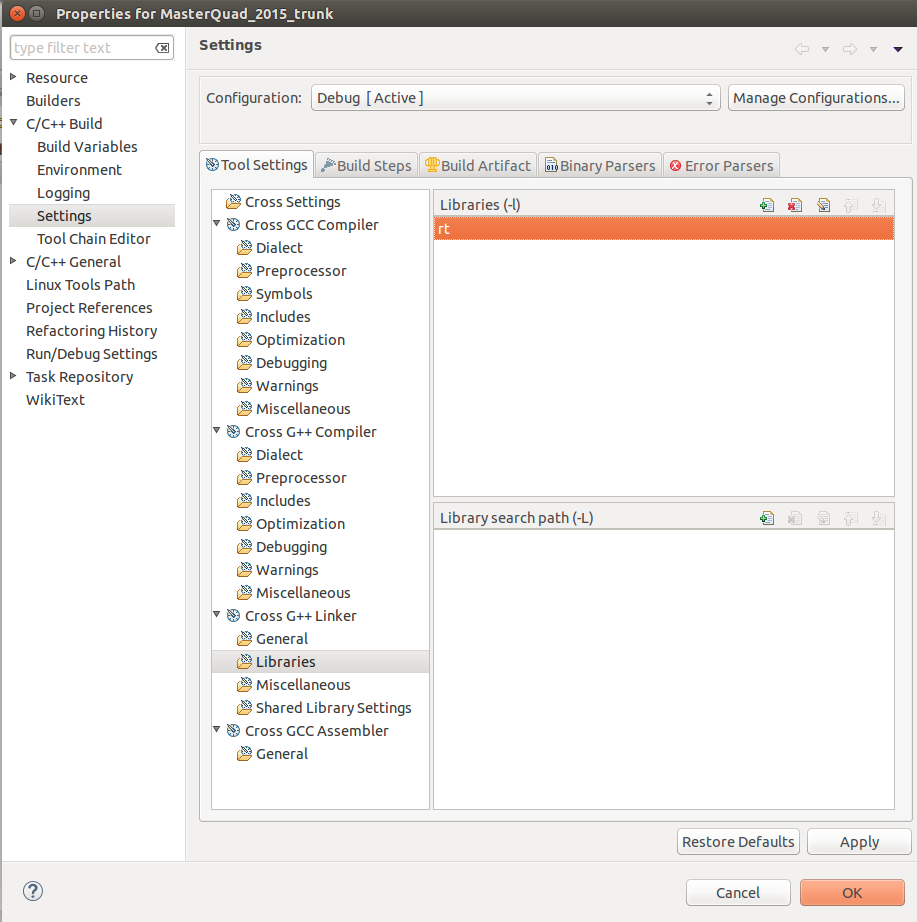
\includegraphics[width=0.5\textwidth]{fig/ch-matlab-lib/projectAddDone}
    \caption[Resulting linker entry with librt]{List of linked libraries of the cross-compiler in Eclipse}
    \label{fig:udpMatlab:udpLib:addDoneSettings}
\end{figure}

For the pre-configured Eclipse Project delivered in the Development Environment of this project the library \texttt{librt} is already correctly linked.

\subsection{Basic network library}
\label{sec:udpMatlab:udpLib:basic}

The network library for this project can be found in \texttt{/impl/trunk/matlab}. The basic functionality is implemented in \texttt{udpLib.h} and \texttt{udpLib.c}, respectively. With \texttt{udpLib}, a UPD-connection can be established and timestamped data packets sent and received.

It is assumed that on both ends of the connection, this library is utilized. Otherwise, it has to be guaranteed, that a symmetric UDP-connection is established. That means, that both machines (local and remote) are using the same port to receive data. This is visulized in fig. \ref{fig:udpMatlab:udpLib:synUdpConnect}.

\begin{figure}[H]
    \centering
    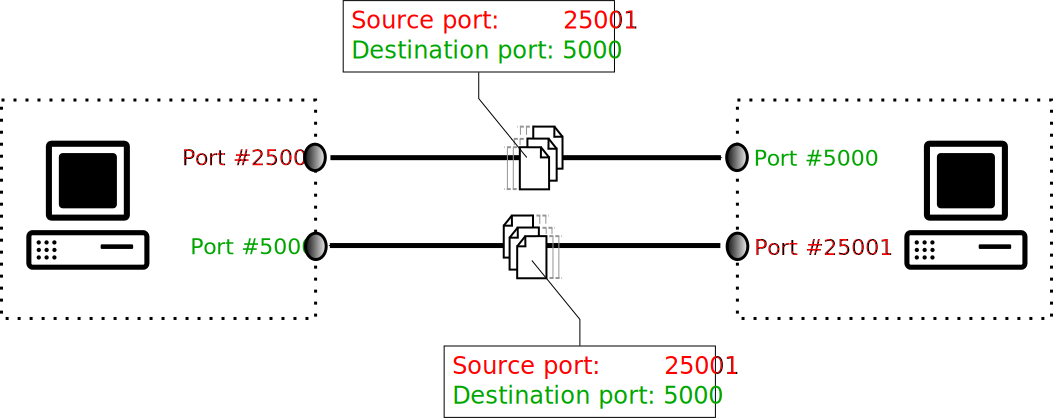
\includegraphics[width=0.85\textwidth]{fig/ch-matlab-lib/symUdpConnect}
    \caption[Symmetric UDP connection setup]{Symmetric UDP connection setup of udpLib. Both machines have the same port numbers for incoming and outgoing traffic opened. In consequence, to reply on an incoming UDP-packet it is sufficient to swap the source and destination IP-address. The port numbers will not change. With this swapped address data, the communication partner gets addressed.}
    \label{fig:udpMatlab:udpLib:synUdpConnect}
\end{figure}

To establish a network connection, the function \texttt{g\_halMatlab\_initConnection\_i32()} has to be called. A IPv4 network address and a destination port has to be given as function parameters. The source port will be chosen automatically. After the connection has been established, data packets can be sent and received by calling \texttt{g\_halMatlab\_sendPacket\_bl()} (without timestamps), respectively \texttt{g\_halMatlab\_recvPacket\_ui32()}. To send packets that are enriched by precise timestamps, the function \texttt{g\_halMatlab\_sendRtPacket\_bl()} can be called. For further details on the stated functions, please consult the code documentation for this project (see also appendix \ref{sec:b-codeDoc}).

To get a simple but comprehensive exemplary code snippet for the usage of the \texttt{udpLib}, the test files (see SVN folder \texttt{/impl/trunk/matlab/tst/}) can be studied. All crucial steps and functions are used there.

To ease the communication with specific data types (raw IMU data as well as data delivered by the sensor fusion), there has been implemented two extensions on the \texttt{udpLib}, shown in chapter \ref{sec:udpMatlab:udpLib:udpImuLib} and chapter \ref{sec:udpMatlab:udpLib:udpSigLib} below.

\subsection{IMU specific network library}
\label{sec:udpMatlab:udpLib:udpImuLib}

To simplify a communication specifically to transmit the raw IMU data from the Raspberry Pi Platform to a MATLAB/Simulink Model, the extended library \texttt{udpImuLib} has been created. Identical to basic \texttt{udpLib}, first of all a UDP-connection has to be established to use the sending and receiving functions. The function \texttt{g\_halMatlab\_initConnection\_i32()} of the library \texttt{udpLib} has to be called.

After a connection has been established, the functions \texttt{g\_halMatlab\_sendImuState\_bl()} and \texttt{g\_halMatlab\_recvImuState\_bl()} can be accessed to send and receive IMU data, marked with a precise timestamp. Different than in the basic \texttt{udpLib}, here shall a structured data variable be given as function parameter. This ensures the order and size of payload data in the UDP-packet and simplifies the parsing of the received data.

The packet data structure can be expanded as shown in listing \ref{code:udpMatlab:udpImuLib:struct} below.

\begin{lstlisting}[caption=C-Code snippet of the expanded IMU data packet structure,label=code:udpMatlab:udpImuLib:struct]
typedef struct{
	/* Timestamp */
	struct
	{
		long int tv_sec;		/* Seconds since Epoch.  */
		long int tv_nsec;		/* Nanoseconds.  */
	} timestamp_st;
	
	/* Raw IMU data */
	struct{
	
		/* Acceleration data (X,Y,Z) */
		struct{
			double	x_f64;	//!< x-component of a 3D vector data
			double	y_f64;	//!< y-component of a 3D vector data
			double	z_f64;	//!< z-component of a 3D vector data
		} acc;
		
		/* Magnetometer data (X,Y,Z) */
		struct{
			double	x_f64;	//!< x-component of a 3D vector data
			double	y_f64;	//!< y-component of a 3D vector data
			double	z_f64;	//!< z-component of a 3D vector data
		} mag;
		
		/* Gyroscope data (yaw,pitch,roll) */
		struct
		{
			double l_yaw_f64;
			double l_pitch_f64;
			double l_roll_f64;
		} gyro;
		
		double temperature_f64;
		double pressure_f64;
		
	}	imuState_st;
	
} halMatlab_rtImuPayload;
\end{lstlisting}

\subsection{Signal Layer specific network library}
\label{sec:udpMatlab:udpLib:udpSigLib}

An additional extension to the \texttt{udpLib} has been implemented, to ease the transmission of sensor fusioned orientation data. For test and validation purposes, the output of the Complementary-Filter and Kalman-Filter has been observed via MATLAB/Simulink (see chapter \ref{sec:sensorFusion}). The extended library \texttt{udpSigLib} eases therefore the network access.

The below shown listing \ref{code:udpMatlab:udpSigLib:struct} shows the expanded data packet structure to transmit orientation data from the Raspberry Pi to a remote machine, and vice versa.

\begin{lstlisting}[caption=C-Code snippet of the expanded Orientation data packet structure,label=code:udpMatlab:udpSigLib:struct]
typedef struct{
	/* Timestamp */
	struct
	{
		long int tv_sec;		/* Seconds since Epoch.  */
		long int tv_nsec;		/* Nanoseconds.  */
	} timestamp_st;
	
	/* Orientation data in space (roll, pitch, yaw) */
	struct{
		double roll_f64;
		double pitch_f64;
		double yaw_f64;
	}	sigState_st;
	
} halMatlab_rtSigPayload;
\end{lstlisting}

Identical to basic \texttt{udpLib}, first of all a UDP-connection has to be established to use the sending and receiving functions. The function \texttt{g\_halMatlab\_initConnection\_i32()} of the library \texttt{udpLib} has to be called.

After a connection has been established, the functions \texttt{g\_halMatlab\_sendSigState\_bl()} and \texttt{g\_halMatlab\_recvSigState\_bl()} can be accessed to send and receive IMU data, marked with a precise timestamp. Different than in the basic \texttt{udpLib}, here shall a structured data variable be given as function parameter as depicted in listing \ref{code:udpMatlab:udpSigLib:struct}. This ensures the order and size of payload data in the UDP-packet and simplifies the parsing of the received data.

Another data structure called \texttt{halMatlab\_rtSigAllStatePayload} is defined in \texttt{udpSigLib} that comprises a precise timestamp, complete raw IMU data and two times the orientation data of the quadrocopter (one output of the Complementary-Filter, another output of the Kalman-Filter). Nevertheless, this data packet structure is considered for test and validation purposes only. It should not be used in an operational (actual flying) code, due to the huge payload of the data packets and the resulting network traffic.

%- - - - - - - - - - - - - - - - - - - - - - 
% Section: MATLAB/Simulnk S-Function Block to receive sensor and filter data
%- - - - - - - - - - - - - - - - - - - - - - 
\section{MATLAB/Simulink S-Function}
\label{sec:udpMatlab:simulinkBlock}

As a counterpart to the C library \texttt{udpLib}, a special block for MATLAB/Simulink is delivered to handle a UDP-connection according to \texttt{udpLib}. To access the network peripherals out of MATLAB/Simulink, a S-Function had to be created that also utilizes the C library \texttt{udpLib} (as shown in chapter \ref{sec:udpMatlab:udpLib}). The complete S-Function block acts as a signal source and provides the received UDP-data packets of a \texttt{udpLib}-connection as time-discrete signals in the Simulink model.

Nevertheless, as the \texttt{udpLib} provides functions to send and receive UDP-Packets, it would also be possible to implement a sink or a block with inputs and outputs to loop data through MATLAB/Simulink. Since during this project the MATLAB/Simulink model has been used for validation purposes only, such complex setups has been not regarded yet.

\subsection{Block creation with S-Function builder}
\label{sec:udpMatlab:simulinkBlock:builder}

To create a Simulink model with a network connection functionality, a S-Function template has to be created, firstly. Together with the template block, a C-Code template will be created that has to be extended by\texttt{udpLib}-function calls. Last but not least, the received data packets have to be parsed and translated into Simulink signals.

As an step-by-step example, a Simulink block to read all raw IMU values via network from the Raspberry Pi shall be created in this section (used version: \texttt{MATLAB R2013a}).

To create easily a S-Function block, the S-Function Builder of MATLAB/Simulink can be used as shown below. First, start MATLAB/Simulink and create a new blank model. Open the Simulink Library Broswer and click on \texttt{Simulink --> User-Defined Functions}, as depicted in fig. \ref{fig:udpMatlab:simulinkBlock:builder:step1} (see marked area '1.').

\begin{figure}[H]
    \centering
    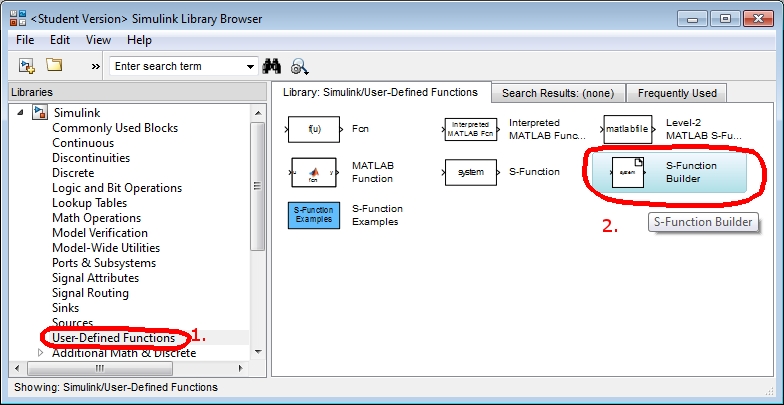
\includegraphics[width=0.75\textwidth]{fig/ch-matlab-lib/sFuncBuilder_matlabLibrary}
    \caption{S-Function Builder 01}
    \label{fig:udpMatlab:simulinkBlock:builder:step1}
\end{figure}

Drag the icon S-Function Builder into your model, such that your model will look similar to fig. \ref{fig:udpMatlab:simulinkBlock:builder:step2}. After you have placed your S-Function Builder block properly, perform a double-click on the newly created Simulink block.

\begin{figure}[H]
    \centering
    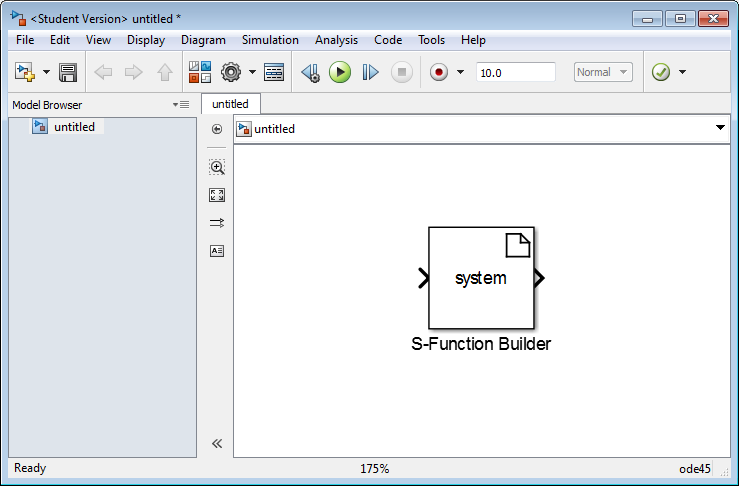
\includegraphics[width=0.75\textwidth]{fig/ch-matlab-lib/sFuncBuilder_matlabModel_00}
    \caption{S-Function Builder 02 (Simulink model)}
    \label{fig:udpMatlab:simulinkBlock:builder:step2}
\end{figure}

A window will pop up, as depicted in fig. \ref{fig:udpMatlab:simulinkBlock:builder:step3}. Choose an appropriate S-Function name (in this example '\texttt{myUdpSource}' is used) and type it in the textbox in top area of the configuration window. Next click on \texttt{Initialization} of the tab menu. You will see four properties \texttt{S-function settings} in the middle of the window. In case you are creating a signal source, as shown in this document, ensure that all state numbers are set to zero!

\textbf{Remark:}\\
Since MATLAB/Simulink treats all Simulink blocks as state space systems, internally, a simple signal source has zero states. The received UDP-packets are simply translated into Simulink signals without further processing. If you want to model a specific system behavior with your S-Function block, you might have some states (usually discrete states, since the UDP-packets will arrive in a time-discrete and isochronous manner).

\begin{figure}[H]
    \centering
    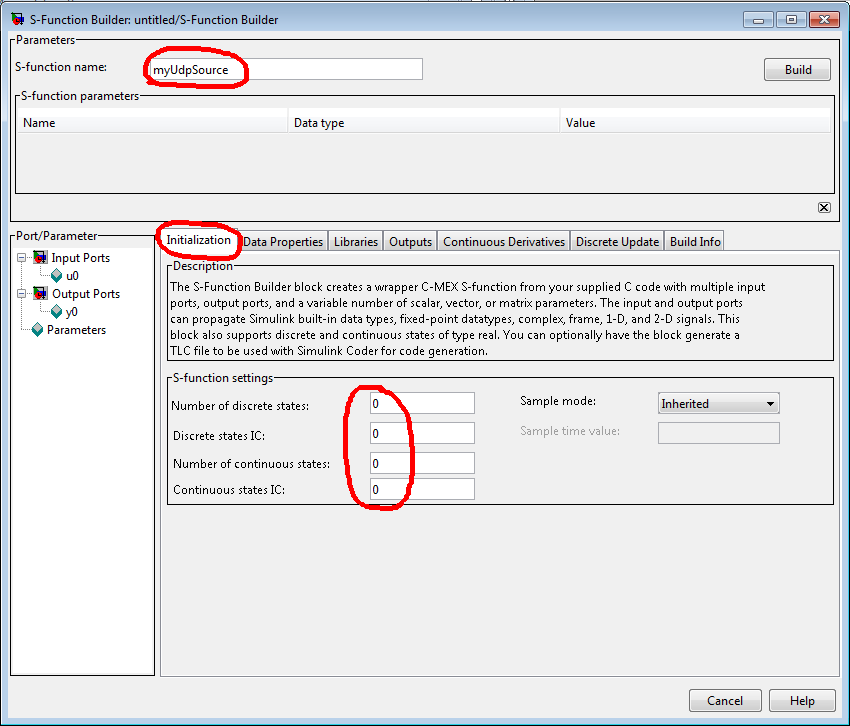
\includegraphics[width=0.7\textwidth]{fig/ch-matlab-lib/sFuncBuilder_matlabBuilder_00}
    \caption{S-Function Builder 03}
    \label{fig:udpMatlab:simulinkBlock:builder:step3}
\end{figure}

Since a signal source shall be created here, the S-Function block does not need to have any inputs. In consequence, all input ports have to be deleted. To edit the signal ports of the S-Function block, click on \texttt{Data Properties} of the tab menu (see fig. \ref{fig:udpMatlab:simulinkBlock:builder:step4a}, mark '1.'). In the middle of the window, a second tab menu called \texttt{Port and Parameter properties} will appear. Select the tab \texttt{Input ports} and delete the default entry.

To delete the default entry, select the entry by clicking on the corresponding row (see fig. \ref{fig:udpMatlab:simulinkBlock:builder:step4a}, mark '2.'). Press the red X-Button to finally delete the entry, as shown in fig. \ref{fig:udpMatlab:simulinkBlock:builder:step4a} (mark '3.').

Now, the output ports of the S-Function block can be defined. Click on the tab \texttt{Output ports}. In case there are any default entries, delete all.

In this example all raw IMU values shall be read via network and fed into the Simulink model. For this purpose, we create for each sensor one output port. It is important to consider that some of the sensors such as accelerometer or gyrosensor will have measurement values for each axis in space (X, Y and Z, respectively roll, pitch and yaw). In consequence, some output ports will have a vector as output type. This will be represented in the \texttt{Rows} value as depicted in fig. \ref{fig:udpMatlab:simulinkBlock:builder:step4b} (see mark '2.')

\begin{figure}[H]
    \centering
    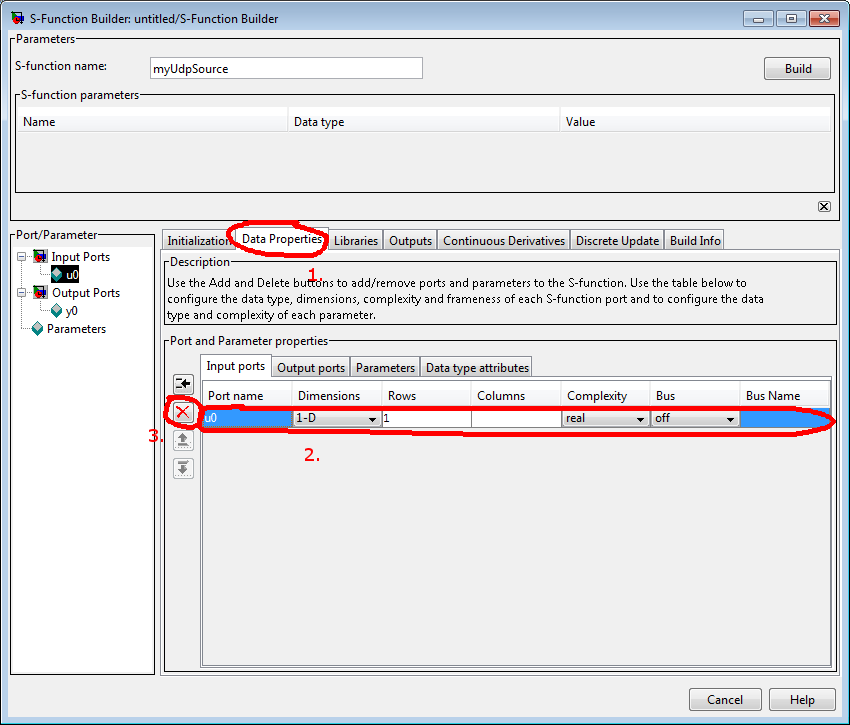
\includegraphics[width=0.7\textwidth]{fig/ch-matlab-lib/sFuncBuilder_matlabModel_01}
    \caption{S-Function Builder 04.a (input ports)}
    \label{fig:udpMatlab:simulinkBlock:builder:step4a}
\end{figure}

For this example, the following output ports shall be added:
\begin{enumerate}
	\item \textbf{Acceleration sensor}:\\
	Port name: \texttt{acc}\\
	Rows:	\texttt{3} (X,Y,Z axis)
	
	\item \textbf{Gyrosensor}:\\
	Port name: \texttt{gyro}\\
	Rows:	\texttt{3} (roll, pitch, yaw)
	
	\item \textbf{Magnetometer}:\\
	Port name: \texttt{mag}\\
	Rows:	\texttt{3} (X,Y,Z axis)
	
	\item \textbf{Barometer}:\\
	Port name: \texttt{baro}\\
	Rows:	\texttt{1} (1-dimensional pressure value)
	
	\item \textbf{Temperature}:\\
	Port name: \texttt{temp}\\
	Rows:	\texttt{1} (1-dimensional temperature)
\end{enumerate}

To add the output port to the S-Function block, click on the Add-Button as shown in fig. \ref{fig:udpMatlab:simulinkBlock:builder:step4b} (mark '1.'). A new row with a blank name will appear. Double-click on the field \texttt{Port name} and enter the first port name as shown in the enumeration above. Since the output signal shall be a vector, the field \texttt{Dimensions} has to remain at the value '\texttt{1-D}'. Double-click on the field \texttt{Rows} and enter corresponding row number (e.g. '3' for the acceleration sensor). The field \texttt{Columns} can be left blank.

Since the IMU values are no complex numbers but completely real numbers so far, the field \texttt{Complexity} has to remain at the value \texttt{real}.

\begin{figure}[H]
    \centering
    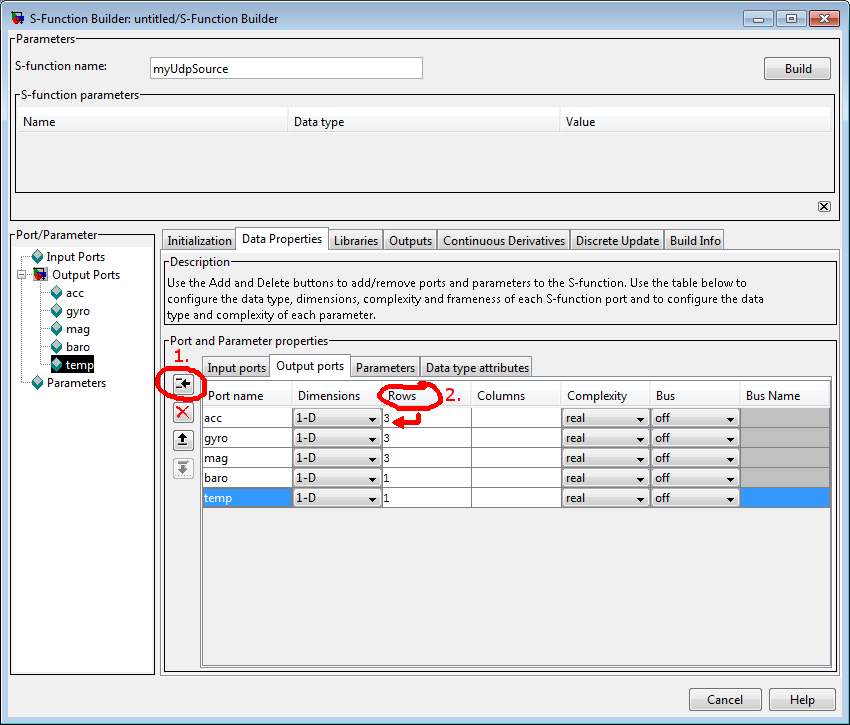
\includegraphics[width=0.7\textwidth]{fig/ch-matlab-lib/sFuncBuilder_matlabBuilder_01}
    \caption{S-Function Builder 04.b (output ports)}
    \label{fig:udpMatlab:simulinkBlock:builder:step4b}
\end{figure}

Proceed this procedure until all output signals are defined. When all sensors are defined, the output ports list should look similar to fig. \ref{fig:udpMatlab:simulinkBlock:builder:step4b}.

Simultaneously to the editing of output ports, the S-Function block in the Simulink model should change its structure of ports. When all output ports have been defined, the S-Function block should look similar to fig. \ref{fig:udpMatlab:simulinkBlock:builder:step4_model}. All output ports are graphically represented and properly named as given by the \texttt{Port name} in the output port list of the S-Function Builder window.

Finally, the build options can be defined. To set the build options, click on the tab \texttt{Build Info} of the main tab menu, as shown in fig. \ref{fig:udpMatlab:simulinkBlock:builder:step5}.

In this example, a network connection has to be established. For that purpose, it is necessary to call the initialization function and close function of the C library \texttt{udpLib} (see chapter \ref{sec:udpMatlab:udpLib}). The network connection shall be established whenever the simulation is started. As soon as the Simulink simulation gets terminated, the network connection shall be closed. Therefore, the corresponding functions \texttt{Start} and \texttt{Terminate} in the S-Function template code has to be provided by the S-Function Builder.

\begin{figure}[H]
    \centering
    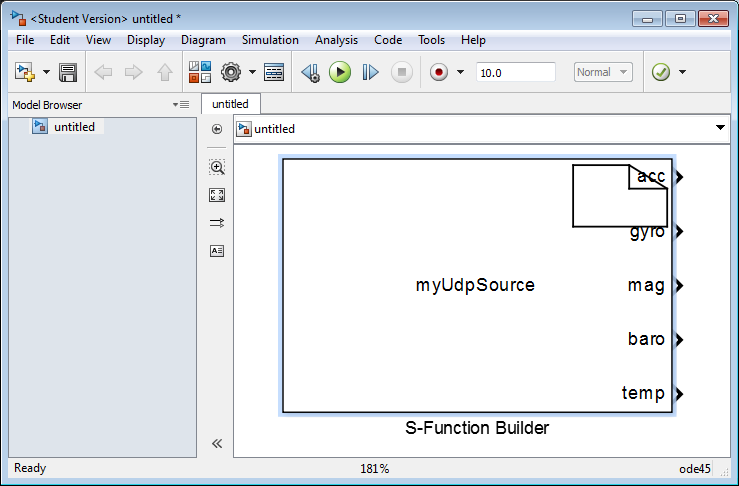
\includegraphics[width=0.7\textwidth]{fig/ch-matlab-lib/sFuncBuilder_matlabModel_toBuilder_01}
    \caption{S-Function Builder 04.b (Simulink model)}
    \label{fig:udpMatlab:simulinkBlock:builder:step4_model}
\end{figure}

\begin{figure}[H]
    \centering
    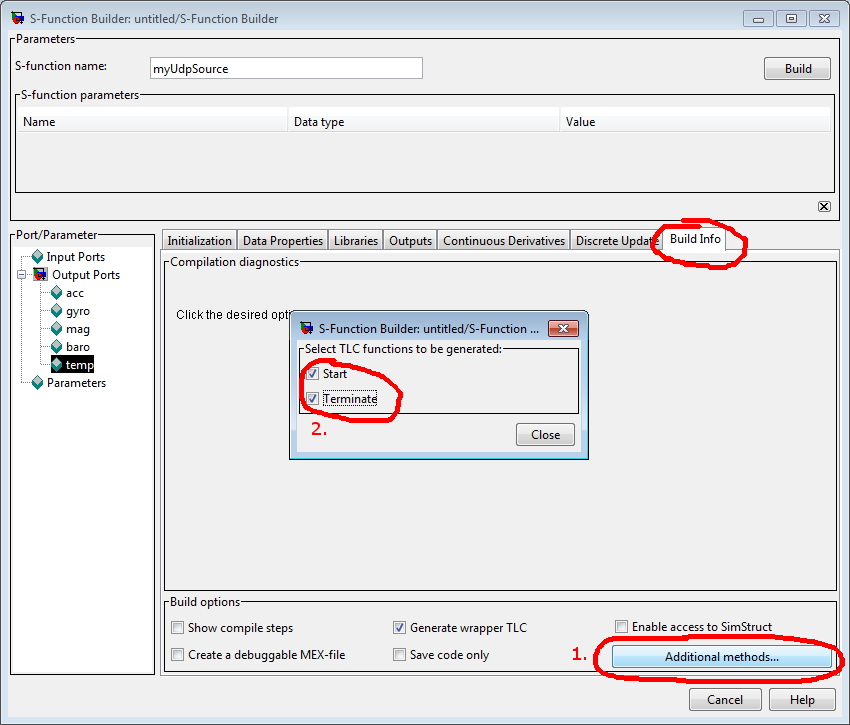
\includegraphics[width=0.7\textwidth]{fig/ch-matlab-lib/sFuncBuilder_matlabBuilder_02}
    \caption{S-Function Builder 05}
    \label{fig:udpMatlab:simulinkBlock:builder:step5}
\end{figure}

To activate the generation of the \texttt{Start} and \texttt{Terminate} function, click on '\texttt{Additional methods...}' at the bottom right corner of the S-Function Builder window (see fig. \ref{fig:udpMatlab:simulinkBlock:builder:step5}, mark '1.'). A new window will pop up. Tick the check marks \texttt{Start} and \texttt{Terminate} in the menu (see fig. \ref{fig:udpMatlab:simulinkBlock:builder:step5}, mark '2.') and press the Close-button.

Optionally, there can be defined some parameters of the S-Function to parametrize the behavior of the Simulink block. To create a parameter for the S-Function, click again on tab \texttt{Data Properties} on the main tab menu (see fig. \ref{fig:udpMatlab:simulinkBlock:builder:step6}, mark '1.'). Navigate to the tab \texttt{Parameters} in the appeared menu (see fig. \ref{fig:udpMatlab:simulinkBlock:builder:step6}, mark '2.'). By default, a emtpy parameter list will appear. Press the Add-Button as depicted in fig. \ref{fig:udpMatlab:simulinkBlock:builder:step6} (mark '3.') and a new entry will appear. Double-click on the field \texttt{Parameter name} and enter 'sampleTime'. For this example, the assumed sample time shall define expected time interval between each UDP packet received from the Raspberry Pi.

To specify a default value for the newly created parameter, click on the field \texttt{Value} of the table \texttt{S-function parameters} on the top of the S-Function Builder window (see fig. \ref{fig:udpMatlab:simulinkBlock:builder:step6}, mark '4.').

\begin{figure}[H]
    \centering
    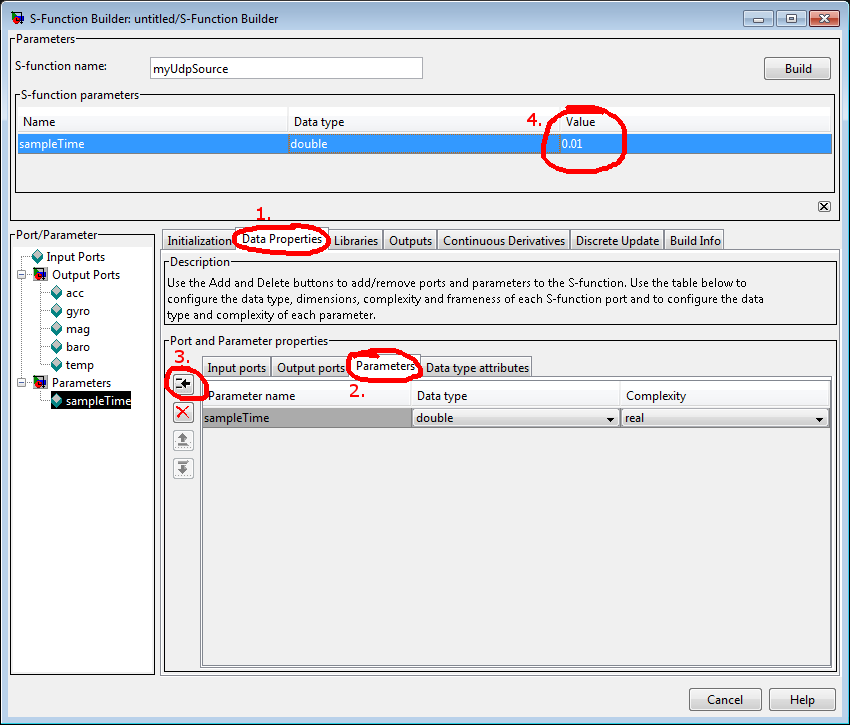
\includegraphics[width=0.7\textwidth]{fig/ch-matlab-lib/sFuncBuilder_matlabBuilder_03optional}
    \caption{S-Function Builder 06 (optional)}
    \label{fig:udpMatlab:simulinkBlock:builder:step6}
\end{figure}

\textbf{Remark:}\\
In this example, the \texttt{Data Type} for the parameter \texttt{sampleTime} has been chosen as \texttt{double}. Although it might be reasonable to choose an integer data type, for convenience and ease of use it is the best choice to use the \texttt{double} data type. MATLAB/Simulink uses the \texttt{double} data type for all signals, internally. In consequence, whenever a user will specify a number (e.g. '\texttt{100}') for a parameter MATLAB will assume to get a double value. If a different data type has been chosen in the S-Function Builder (e.g. \texttt{uint8}), the user will have to type '\texttt{uint8(100)}'. Otherwise, a data type error will pop up and the user-defined parameter will not be accepted.

\begin{figure}[H]
    \centering
    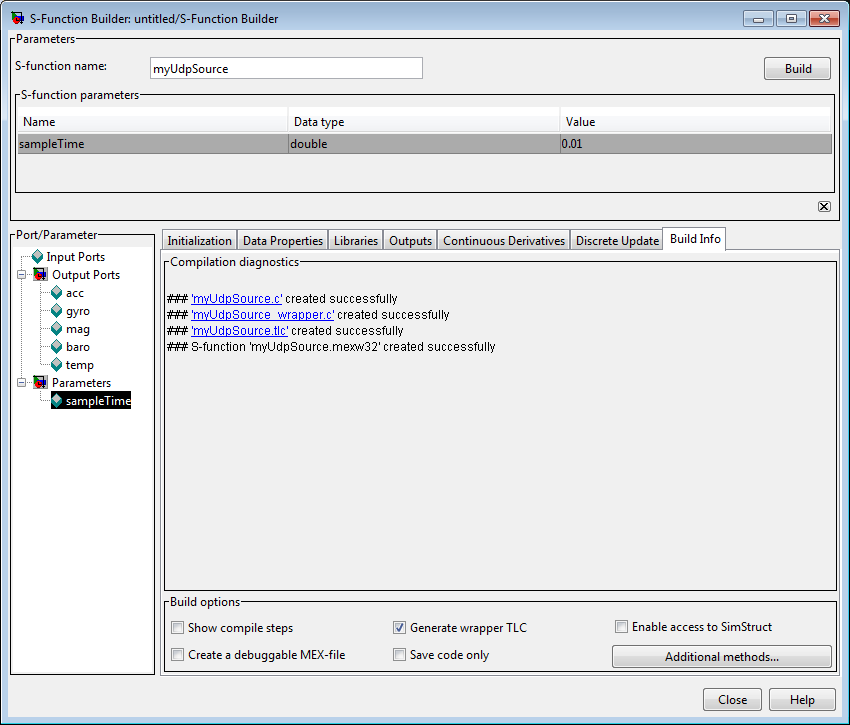
\includegraphics[width=0.7\textwidth]{fig/ch-matlab-lib/sFuncBuilder_matlabBuilder_04_success}
    \caption{S-Function Builder 07}
    \label{fig:udpMatlab:simulinkBlock:builder:step7}
\end{figure}

When all parameters and settings have been defined, the button \texttt{Build} in the top right corner of the S-Function Builder window can be pressed. The S-Function Builder will create all necessary files, such as the C-Code template files \texttt{myUdpSource.c} as well as \texttt{myUdpSource\_wrapper.c}.

If the template generation was successful, the S-Function Builder window will look similar to fig. \ref{fig:udpMatlab:simulinkBlock:builder:step7}. The S-Function Builder window can be closed now, by clicking on the Close-Button in the bottom right corner.

\subsection{Extending the C-Code templates}
\label{sec:udpMatlab:simulinkBlock:extendTemplates}

As a next step, the C-Code template files have to be extended to the needs of the required functionality of the S-Function block. In the case of this example, the \texttt{udpLib} library has to be included and the corresponding functions have to called in an appropriate way. A network connection shall be established whenever the Simulink simulation is started. Furthermore, the network connection shall be closed whenever the Simulink simulation has terminated. Last but not least, whenever a UDP packet is received, the data shall be extracted and transferred to the Simulink model as Simulink signals.

First, the C-Code file \texttt{myUdpSource.c} shall be edited. The complete C-Code template generated by the S-Function Builder can be found in Appendix \ref{sec:c-sFunc-Code:rawTemplate}. Open the file in the preferred IDE or MATLAB.

In the top of the file, a large block comment and a long list of \texttt{define} statements can be found. According to listing \ref{code:c-sFunc-Code:rawTemplate}, after line 148 all defines have been stated. To access the network functionalities, insert here an \texttt{include} statement of the \texttt{udpImuLib} (in this example the library \texttt{udpImuLib} shall be included since all raw IMU values shall be read). Additionally to the \texttt{include} statement, two \texttt{define} statements ( \texttt{REMOTE\_HOST\_IPADDR} and \texttt{REMOTE\_HOST\_PORT} ) shall be inserted to define the remote host IPv4 address as well as the listen/destination port number (see line 151l. of listing \ref{code:udpMatlab:simulinkBlock:extendTemplates:includeUdpLib}). Since the udpLib establishes a symmetric UDP connection, the listen port number and the destination port number will be identical (see chapter \ref{sec:udpMatlab:udpLib}). Lastly, an integer variable \texttt{int m\_simSocketNumber} shall be declared to store the socket number of the UDP-connection.

\begin{lstlisting}[caption={[\texttt{myUdpSource.c} extended by include statement]C-Code template file 'myUdpSource.c' extended by a include statement to link the \texttt{udpLib} library (code snippet of listing \ref{code:c-sFunc-Code:rawTemplate}, lines 143 ll.)},label=code:udpMatlab:simulinkBlock:extendTemplates:includeUdpLib,firstnumber=143]
/*<<<<<<<<<<<<<<<<<<<<<<<<<<<<<<<<<<<<<<<<<<<<<<<<<<<<<<<<<<<<<<<<<*/
#include "simstruc.h"
#define PARAM_DEF0(S) ssGetSFcnParam(S, 0)

#define IS_PARAM_DOUBLE(pVal) (mxIsNumeric(pVal) && !mxIsLogical(pVal) && !mxIsEmpty(pVal) && !mxIsSparse(pVal) && !mxIsComplex(pVal) && mxIsDouble(pVal))

#include "../path/to/udpLib/udpImuLib.h"

#define REMOTE_HOST_IPADDR	{192,168,22,161}
#define REMOTE_HOST_PORT		5000

static int m_simSocketNumber 	= 0;

extern void myUdpSource_Outputs_wrapper(real_T *acc,
																				real_T *gyro,
																				real_T *mag,
																				real_T *baro,
																				real_T *temp, 
																				const real_T  *sampleTime, 
																				const int_T p_width0);
\end{lstlisting}

The changed code will look similar to listing \ref{code:udpMatlab:simulinkBlock:extendTemplates:includeUdpLib} as shown below. In the shown code snippet, the path to the \texttt{udpImuLib} is expressed with the placeholder '\texttt{../path/to/udpLib}'. Change this placeholder to a relative path according to the folder structure used in your project.

Next, the network connection shall be established whenever the Simulink simulation gets started. Starting at line 267 of the raw C-Code template (see listing \ref{code:c-sFunc-Code:rawTemplate}) the function \texttt{mdlStart} is defined. In the function body two local variables to store the IPv4 address and the listen port number shall be defined. Furthermore, the function \texttt{g\_halMatlab\_initConnection\_i32()} of the C library \texttt{udpLib} shall be called. The returned socket number shall be stored to \texttt{m\_simSocketNumber}, as defined in listing \ref{code:udpMatlab:simulinkBlock:extendTemplates:includeUdpLib}. Optionally, a \texttt{printf} statement can be inserted for debugging purposes. The completed function body can be seen in listing \ref{code:udpMatlab:simulinkBlock:extendTemplates:startFunc} below.

\begin{lstlisting}[caption={[\texttt{myUdpSource.c} extended by start function code]C-Code template file 'myUdpSource.c' extended by the function body of the \texttt{mdlStart} function (code snippet of listing \ref{code:c-sFunc-Code:rawTemplate}, lines 265 ll.)},label=code:udpMatlab:simulinkBlock:extendTemplates:startFunc,firstnumber=265]
#define MDL_START  /* Change to #undef to remove function */
#if defined(MDL_START) 
  /* Function: mdlStart =======================================================
   * Abstract:
   *    This function is called once at start of model execution. If you
   *    have states that should be initialized once, this is the place
   *    to do it.
   */
  static void mdlStart(SimStruct *S)
  {
		unsigned char 	remoteIpAddr[4] = REMOTE_HOST_IPADDR;
    unsigned short 	listenPort 			= REMOTE_HOST_PORT;
    
		printf("Listening to port %d\n",listenPort);
	  
    m_simSocketNumber = g_halMatlab_initConnection_i32( remoteIpAddr,
																												listenPort);
  }
#endif /*  MDL_START */
\end{lstlisting}

As a next step, the network connection shall be closed whenever the Simulink simulation gets terminated. For that purpose, the function \texttt{g\_halMatlab\_closeSocket\_bl()} shall be called. The function parameter will be the stored socket number \texttt{m\_simSocketNumber}. Depending on the boolean return state of the function \texttt{g\_halMatlab\_closeSocket\_bl()}, a text output of the success or error shall be given to the user. The complete function body can be seen in listing \ref{code:udpMatlab:simulinkBlock:extendTemplates:termFunc} below.

\begin{lstlisting}[caption={[\texttt{myUdpSource.c} extended by terminate function code]C-Code template file 'myUdpSource.c' extended by the function body of the \texttt{mdlTerminate} function (code snippet of listing \ref{code:c-sFunc-Code:rawTemplate}, lines 307 ll.)},label=code:udpMatlab:simulinkBlock:extendTemplates:termFunc,firstnumber=307]
/* Function: mdlTerminate =====================================================
 * Abstract:
 *    In this function, you should perform any actions that are necessary
 *    at the termination of a simulation.  For example, if memory was
 *    allocated in mdlStart, this is the place to free it.
 */
static void mdlTerminate(SimStruct *S)
{
	if ( g_halMatlab_closeSocket_bl(m_simSocketNumber) )
	{
		// true state refers to occurrence of errors
		printf("Could not close the network socket\n");
	}
	else
	{
		// false state refers to absence of errors
		printf("Network socket successfully closed\n");
	}
}
\end{lstlisting}

If the code template has been generated with custom block parameters (see chapter \ref{sec:udpMatlab:simulinkBlock:builder}, especially fig. \ref{fig:udpMatlab:simulinkBlock:builder:step6}), the parameter \texttt{sampleTime} of this example can be used to set the default sample time of the S-Function block. Starting at line 254 of the raw C-Code template (see listing \ref{code:c-sFunc-Code:rawTemplate}) the function \texttt{mdlInitializeSampleTimes()} is defined. To adjust the default sample time to the user defined sample time, the called function \texttt{ssSetSampleTime(S, 0, SAMPLE\_TIME\_0)} (line 260 of listing \ref{code:c-sFunc-Code:rawTemplate}) has to be adapted. The user-defined sample time has to be extracted out of the parameter list. The complete function body of \texttt{mdlInitializeSampleTimes()} can be seen in listing \ref{code:udpMatlab:simulinkBlock:extendTemplates:sampleTimeFunc} below.

\begin{lstlisting}[caption={[\texttt{myUdpSource.c} extended by user-defined sample time]C-Code template file 'myUdpSource.c' extended by a user-defined sample time via block parameters (code snippet of listing \ref{code:c-sFunc-Code:rawTemplate}, lines 254 ll.)},label=code:udpMatlab:simulinkBlock:extendTemplates:sampleTimeFunc,firstnumber=254]
/* Function: mdlInitializeSampleTimes =========================================
 * Abstract:
 *    Specifiy  the sample time.
 */
static void mdlInitializeSampleTimes(SimStruct *S)
{
    double* l_sampleTimePtr;
    
    //get sample time, configured in block parameters
    l_sampleTimePtr = mxGetPr( ssGetSFcnParam(S, 0) );
		
		//output for debugging purposes
    printf("Set sampling time to %lf\n",*l_sampleTimePtr);
    
		//cast double type to time_T type
    ssSetSampleTime(S, 0, (time_T)*l_sampleTimePtr );
    ssSetOffsetTime(S, 0, 0.0);
}
\end{lstlisting}

Now, the file \texttt{myUdpSource.c} is ready and fully functional to the needs of this example. The \texttt{udpLib} is successfully linked and a UDP-connection gets established and closed, accordingly to the state of the Simulink simulation. Still missing is the crucial part of receiving and translating UDP-packets to Simulink signals.

In line 302 of the raw C-Code template (see listing \ref{code:c-sFunc-Code:rawTemplate}), to translate the output signals the external function \texttt{myUdpSource\_Outputs\_wrapper()} gets called. This function is defined in the file \texttt{myUdpSource\_wrapper.c}. Unfortunately for this example, the pre-defined interface does not fulfill all needs for the network access fnctionality. Since a network packet shall be received inside of the outputs wrapper function, the socket number of the connection has to be known. Therefore, the function parameter list of \texttt{myUdpSource\_Outputs\_wrapper()} shall be extended by an integer number \texttt{int socketNum}. For this purpose, the file \texttt{myUdpSource.c} has to be altered in two lines. The declaration as well as the call of the external function \texttt{myUdpSource\_Outputs\_wrapper()} in line 149 and line 302, respectively, of the raw C-Code template has to be altered to the new function parameter list. The changed code-snippets of \texttt{myUdpSource.c} can be seen in listing \ref{code:udpMatlab:simulinkBlock:extendTemplates:changedWrapperDec} and listing \ref{code:udpMatlab:simulinkBlock:extendTemplates:changedWrapperCall} below.

\begin{lstlisting}[caption={[\texttt{myUdpSource.c}, changed declaration of \texttt{myUdpSource\_Outputs\_wrapper()}]C-Code template file 'myUdpSource.c' with changed declaration of the external function \texttt{myUdpSource\_Outputs\_wrapper()} (code snippet of listing \ref{code:c-sFunc-Code:rawTemplate}, lines 149 ll.)},label=code:udpMatlab:simulinkBlock:extendTemplates:changedWrapperDec,firstnumber=149]
extern void myUdpSource_Outputs_wrapper(real_T *acc,
                                        real_T *gyro,
                                        real_T *mag,
                                        real_T *baro,
                                        real_T *temp, 
                                        const real_T  *sampleTime,
                                        const int_T p_width0,
                                        int socketNum);
\end{lstlisting}

\begin{lstlisting}[caption={[\texttt{myUdpSource.c} with changed call of \texttt{myUdpSource\_Outputs\_wrapper()}]C-Code template file 'myUdpSource.c' with changed call of the external function \texttt{myUdpSource\_Outputs\_wrapper()} inside the function body of function \texttt{mdlOutputs} (code snippet of listing \ref{code:c-sFunc-Code:rawTemplate}, lines 289 ll.)},label=code:udpMatlab:simulinkBlock:extendTemplates:changedWrapperCall,firstnumber=289]
/* Function: mdlOutputs =======================================================
 *
*/
static void mdlOutputs(SimStruct *S, int_T tid)
{
    real_T        *acc  = (real_T *)ssGetOutputPortRealSignal(S,0);
    real_T        *gyro  = (real_T *)ssGetOutputPortRealSignal(S,1);
    real_T        *mag  = (real_T *)ssGetOutputPortRealSignal(S,2);
    real_T        *baro  = (real_T *)ssGetOutputPortRealSignal(S,3);
    real_T        *temp  = (real_T *)ssGetOutputPortRealSignal(S,4);
    const int_T   p_width0  = mxGetNumberOfElements(PARAM_DEF0(S));
    const real_T  *sampleTime  = (const real_T *)mxGetData(PARAM_DEF0(S));

    myUdpSource_Outputs_wrapper(acc,
																gyro, 
																mag, 
																baro, 
																temp, 
																sampleTime, 
																p_width0, 
																m_simSocketNumber);
}
\end{lstlisting}

Finally, the definition of the function \texttt{myUdpSource\_Outputs\_wrapper()} in the C-Code file \texttt{myUdpSource\_wrapper.c} has to be adapted to meet the new interface definition as well as implement required network access functionality.

In listing \ref{code:udpMatlab:simulinkBlock:extendTemplates:wrapperExtendInclude}, the \texttt{include} statement has been added to the file \texttt{myUdpSource\_wrapper.c} to access the network functions of the \texttt{udpImuLib} library. In the shown code snippet, the path to the \texttt{udpImuLib} is expressed with the placeholder '\texttt{../path/to/udpLib}'. Change this placeholder to a relative path according to the folder structure used in your project.

\begin{lstlisting}[caption={[\texttt{myUdpSource\_wrapper.c} with added include]C-Code template file 'myUdpSource\_wrapper.c' with added include statement for \texttt{udpImuLib} library (code snippet of listing \ref{code:c-sFunc-Code:rawTemplateWrapper}, lines 36 ll.)},label=code:udpMatlab:simulinkBlock:extendTemplates:wrapperExtendInclude,firstnumber=36]
/* %%%-SFUNWIZ_wrapper_includes_Changes_BEGIN --- EDIT HERE TO _END */
#include <math.h>
#include "../path/to/udpLib/udpImuLib.h"
/* %%%-SFUNWIZ_wrapper_includes_Changes_END --- EDIT HERE TO _BEGIN */
\end{lstlisting}

In listing \ref{code:udpMatlab:simulinkBlock:extendTemplates:wrapperExtendFunc}, the outputs wrapper function \texttt{myUdpSource\_Outputs\_wrapper()} is extended by the call of the network access function \texttt{g\_halMatlab\_recvImuState\_bl()} of the \texttt{udpImuLib} library. This function receives a UDP packet and stores the payload in a structured variable. With this variable, all sent data can be easily translated to the Simulink signals.

Since the Simlink port \texttt{acc}, \texttt{gyro} and \texttt{mag} are output vectors with three rows (as defined in chapter \ref{sec:udpMatlab:simulinkBlock:builder}) the variables can be access as C-Arrays. This can be seen in listing \ref{code:udpMatlab:simulinkBlock:extendTemplates:wrapperExtendFunc}, line 82 ll.

\begin{lstlisting}[caption={[\texttt{myUdpSource\_wrapper.c} with implemented wrapper function]C-Code template file 'myUdpSource\_wrapper.c' with extended and implemented wrapper function \texttt{myUdpSource\_Outputs\_wrapper()} (code snippet of listing \ref{code:c-sFunc-Code:rawTemplateWrapper}, lines 49 ll.)},label=code:udpMatlab:simulinkBlock:extendTemplates:wrapperExtendFunc,firstnumber=49]
/*
 * Output functions
 *
 */
void myUdpSource_Outputs_wrapper(real_T *acc,
                                 real_T *gyro,
                                 real_T *mag,
                                 real_T *baro,
                                 real_T *temp, 
                                 const real_T  *sampleTime, 
                                 const int_T p_width0,
                                 int socketNum)
{
/* %%%-SFUNWIZ_wrapper_Outputs_Changes_BEGIN --- EDIT HERE TO _END */
	
		// define payload structure of UDP packets
    halMatlab_rtImuPayload l_udpPayload_st;
    
		// get a new packet
    l_udpPayload_st = g_halMatlab_recvImuState_bl( socketNum );
    
		// print remote system time for debugging purposes here
    printf("Remote time: %ld.%ld\n",
						l_udpPayload_st.timestamp_st.tv_sec,
						l_udpPayload_st.timestamp_st.tv_nsec);
    
		/* translate the UDP packet data to simulink signals
		 * Remark: Since all used data of the UDP packets are
		 *         already of the type double (see f64 postfix)
		 *         the data is already matching the double
		 *         type data representation, used by MATLAB
		 *         internally.
		 */
    acc[0] = l_udpPayload_st.imuState_st.acc.x_f64;
    acc[1] = l_udpPayload_st.imuState_st.acc.y_f64;
    acc[2] = l_udpPayload_st.imuState_st.acc.z_f64;
    
    gyro[0] = l_udpPayload_st.imuState_st.gyro.l_roll_f64;
    gyro[1] = l_udpPayload_st.imuState_st.gyro.l_pitch_f64;
    gyro[2] = l_udpPayload_st.imuState_st.gyro.l_yaw_f64;
    
    mag[0] = l_udpPayload_st.imuState_st.mag.x_f64;
    mag[1] = l_udpPayload_st.imuState_st.mag.y_f64;
    mag[2] = l_udpPayload_st.imuState_st.mag.z_f64;
    
    baro[0] = l_udpPayload_st.imuState_st.pressure_f64;
    
    temp[0] = l_udpPayload_st.imuState_st.temperature_f64;
/* %%%-SFUNWIZ_wrapper_Outputs_Changes_END --- EDIT HERE TO _BEGIN */
}
\end{lstlisting}

Now all the C-Code of the S-Function block has been adapted according to the requirements of this example. As a final step, the S-Function shall be compiled in MATLAB.

\subsection{Compiling the S-Function block}
\label{sec:udpMatlab:simulinkBlock:compiling}

In order to use the custom S-Function block, created in chapter \ref{sec:udpMatlab:simulinkBlock:builder} and chapter \ref{sec:udpMatlab:simulinkBlock:extendTemplates}, so far, the C-Code has to be compiled with the MATLAB Compiler \texttt{mex}.

For that purpose, change to the MATLAB main window and change current working directory to the location of the S-Function's C-Code files. This can be done either by navigating through the \texttt{Current Folder} window or by typing '\texttt{cd ../path/to/sFuncCode}' in MATLAB's \texttt{Command Window}.

If the MATLAB compiler never has been used on the system, it might be necessary to configure the compilation environment in MATLAB first. To do so, type \texttt{mex -setup} in the \texttt{Command Window}. Plenty of text will appear, similar to listing \ref{code:udpMatlab:simulinkBlock:compiling:mexSetup1} below. MATLAB will ask if it shall search for installed compatible compilers. Answer that question with \texttt{yes}.

\begin{lstlisting}[language=MATLAB,caption=Configuration of MATLAB's mex compiler (part 1),label=code:udpMatlab:simulinkBlock:compiling:mexSetup1]
>> mex -setup
 
Welcome to mex -setup.  This utility will help you set up  
a default compiler.  For a list of supported compilers, see  
http://www.mathworks.com/support/compilers/R2013a/win32.html 
 
Please choose your compiler for building MEX-files: 
 
Would you like mex to locate installed compilers [y]/n? y
\end{lstlisting}

If the used host system is a Windows Operating System and a Microsoft Visual Studio Compiler has been found (as shown in the listing \ref{code:udpMatlab:simulinkBlock:compiling:mexSetup2} below), it is highly recommended to use the Microsoft Visual Studio Compiler for performance and ease of use purposes. Furthermore, it is possible to attach the Microsoft Visual Studio Compiler to the custom S-Function Code (Debugger gets actually attached to \texttt{Matlab.exe}) and debug the C-Code during run-time.

\begin{lstlisting}[language=MATLAB,caption=Configuration of MATLAB's mex compiler (part 2),label=code:udpMatlab:simulinkBlock:compiling:mexSetup2]
Select a compiler: 
[1] Lcc-win32 C 2.4.1 in C:\MATLAB\R2013A~1\sys\lcc 
[2] Microsoft Visual C++ 2010 in C:\Program Files (x86)\Microsoft Visual Studio 10.0 
 
[0] None 
 
Compiler: 2
 
Please verify your choices: 
 
Compiler: Microsoft Visual C++ 2010  
Location: C:\Program Files (x86)\Microsoft Visual Studio 10.0 
 
Are these correct [y]/n? y
 
*************************************************************************** 
  Warning: MEX-files generated using Microsoft Visual C++ 2010 require 
           that Microsoft Visual Studio 2010 run-time libraries be  
           available on the computer they are run on. 
           If you plan to redistribute your MEX-files to other MATLAB 
           users, be sure that they have the run-time libraries. 
*************************************************************************** 
 
 
Trying to update options file: C:\Users\aUserName\AppData\Roaming\MathWorks\MATLAB\R2013a\mexopts.bat 
From template:              C:\MATLAB\R2013A~1\bin\win32\mexopts\msvc100opts.bat 
 
Done . . . 
 
************************************************************************** 
  Warning: The MATLAB C and Fortran API has changed to support MATLAB 
           variables with more than 2^32-1 elements.  In the near future 
           you will be required to update your code to utilize the new 
           API. You can find more information about this at: 
           http://www.mathworks.com/help/matlab/matlab_external/upgrading-mex-files-to-use-64-bit-api.html  
           Building with the -largeArrayDims option enables the new API. 
************************************************************************** 
 
>>
\end{lstlisting}

After the MEX compiler has been successfully configured, the S-Function code can be compiled. For this purpose, type the command \texttt{mex} into the \texttt{Command Window}, followed by each C-Code file used by the S-Function code (also included libraries)! For the S-Function created in this example, the complete call of the MEX compiler will look like shown below.
\begin{lstlisting}[language=MATLAB]
>> mex myUdpSource.c myUdpSource_wrapper.c ../path/to/udpLib/*.c
\end{lstlisting}

%- - - - - - - - - - - - - - - - - - - - - - 
% Section: 3D-Representation of orientation data
%- - - - - - - - - - - - - - - - - - - - - - 
\section{3D-Representation of orientation data}
\label{sec:udpMatlab:orientation3D}

Since this UDP-based network connection to MATLAB is mainly used for testing and validation purposes, a graphical 3D output of the orientation angles produced by the functional unit \texttt{orientation} (see also chapter \ref{sec:sensorFusion}) was required.

To visualize such a 3D representation of the Quadrocopter's orientation angles in space, the authors of this document have chosen a 3-dimensional plane that can be rotated in each rotational axis in space, representing the pitch, roll and yaw angles. For that purpose, a separate User-defined Simulink was created - based on a MATLAB-Function Block. In contrast to a S-Function block, the behavior of a MATLAB-Function block is defined by MATLAB code instead of C-Code. That simplifies the implementation of a specifically needed behavior, e.g. for Rapid Prototyping, at the cost of performance.

\begin{figure}[H]
    \centering
    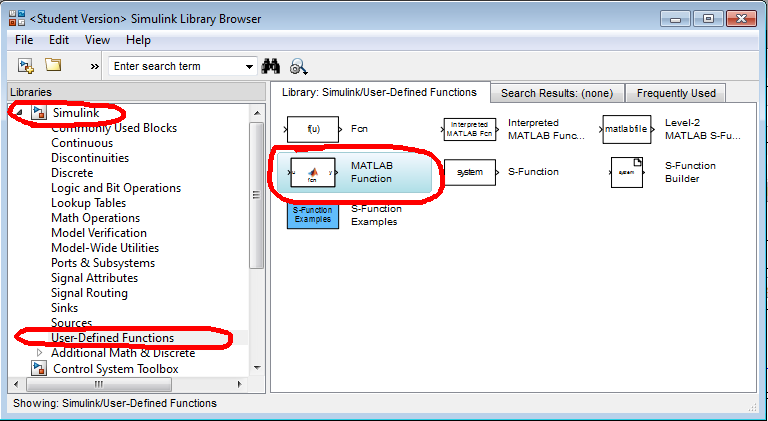
\includegraphics[width=0.85\textwidth]{fig/ch-matlab-lib/matlabFunction}
    \caption{MATLAB-Function Block in Simulink Library Browser}
    \label{fig:udpMatlab:orientation3D:mFunc}
\end{figure}

The create a 3D visualization of the orientation angles, open a Simulink model. Open the Simulink Library Browser and click on \texttt{Simulink --> User-Defined Functions}, as depicted in fig. \ref{fig:udpMatlab:orientation3D:mFunc}. Now drag the MATLAB-Function icon to the Simulink model under development.

\begin{figure}[H]
    \centering
    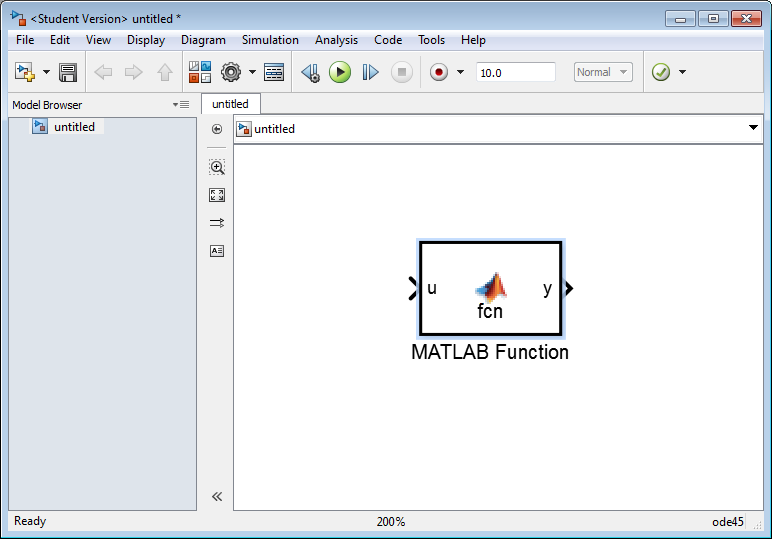
\includegraphics[width=0.7\textwidth]{fig/ch-matlab-lib/matlabFunctionInModel}
    \caption{MATLAB-Function Block in a Simulink model}
    \label{fig:udpMatlab:orientation3D:mFuncInModel}
\end{figure}

When the MATLAB-Function has been dragged into the model, the Simulink window should look similar to fig. \ref{fig:udpMatlab:orientation3D:mFuncInModel}. Double-click on the MATLAB Function block. A new MATLAB code section will appear in the MATLAB Editor with an empty function body. Copy the complete code of listing \ref{code:d-mFunc-Code:3dViz} in the Appendix \ref{sec:d-mFunc-Code} and paste it into recently popped up MATLAB Editor, replacing the default code. Press the save button and check the Simulink model for any changes. The MATLAB Function block should now look similar to fig. \ref{fig:udpMatlab:orientation3D:mFuncInModelFinished} and is called \texttt{drawBox}, according to the function name of the copied MATLAB code of listing \ref{code:d-mFunc-Code:3dViz}.

\begin{figure}[H]
    \centering
    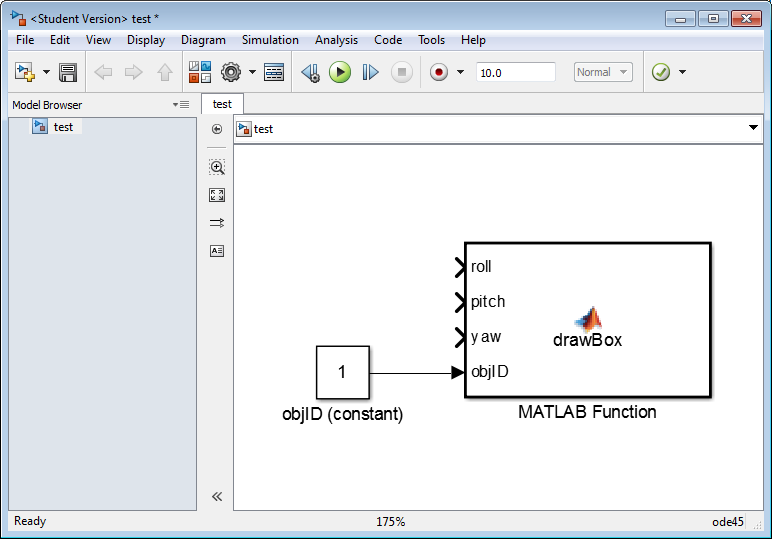
\includegraphics[width=0.85\textwidth]{fig/ch-matlab-lib/matlabFunctionInModel_finished}
    \caption{MATLAB-Function Block for 3D visualization in a Simulink model}
    \label{fig:udpMatlab:orientation3D:mFuncInModelFinished}
\end{figure}

As already depicted in fig. \ref{fig:udpMatlab:orientation3D:mFuncInModelFinished}, the port \texttt{objID} needs to be connected to a constant value block. The constant value has to be a unique number in the range 1 to 3 (the max. range is defined by variable \texttt{objIDMax} of listing \ref{code:d-mFunc-Code:3dViz}, line 24). This number has to be unique among all identical \texttt{drawBox} blocks. This is needed for the internal identification of the window ID and plot ID.

Now the remaining inputs \texttt{roll}, \texttt{pitch} and \texttt{yaw} can be connected to some signal source, providing an angular value with the unit \texttt{degree}. When the model is run, an graphical output as shown in fig. \ref{fig:udpMatlab:orientation3D:mFuncInModelOutput} will appear. According to the angular values of the input ports \texttt{roll}, \texttt{pitch} and \texttt{yaw}, the 3-dimensional plane will rotate as shown in fig. \ref{fig:udpMatlab:orientation3D:mFuncInModelOutputRot}

\begin{figure}[H]
    \centering
    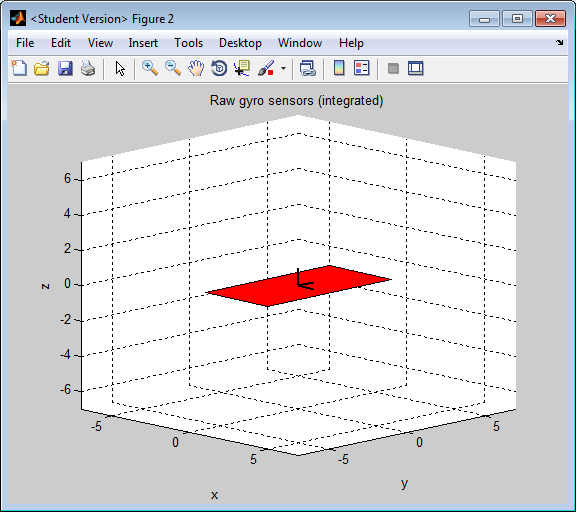
\includegraphics[width=0.65\textwidth]{fig/ch-matlab-lib/matlabFunctionInModel_output}
    \caption{3D graph of the MATLAB-Function Block for 3D visualization}
    \label{fig:udpMatlab:orientation3D:mFuncInModelOutput}
\end{figure}

\begin{figure}[H]
    \centering
    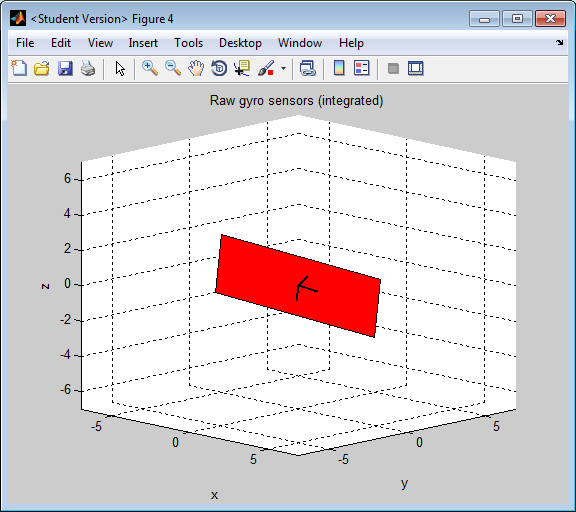
\includegraphics[width=0.65\textwidth]{fig/ch-matlab-lib/matlabFunctionInModel_outputRot}
    \caption{3D graph of the MATLAB-Function Block for 3D visualization (in motion)}
    \label{fig:udpMatlab:orientation3D:mFuncInModelOutputRot}
\end{figure}